The system recognizes two kind of gestures (see also
\ref{fig:gesturesToRecognize}):
\begin{itemize}
  \item A circle that starts from the bottom and runs clockwise
  \item A circle that starts from the bottom and runs counter-clockwise
\end{itemize}
The first gesture is used to mark an item as ``added to cart'' while the second
one serves to switch through the items on the shopping list.

\begin{figure}[h]
\captionsetup{justification=centering}
\begin{subfigure}{0.475\textwidth}
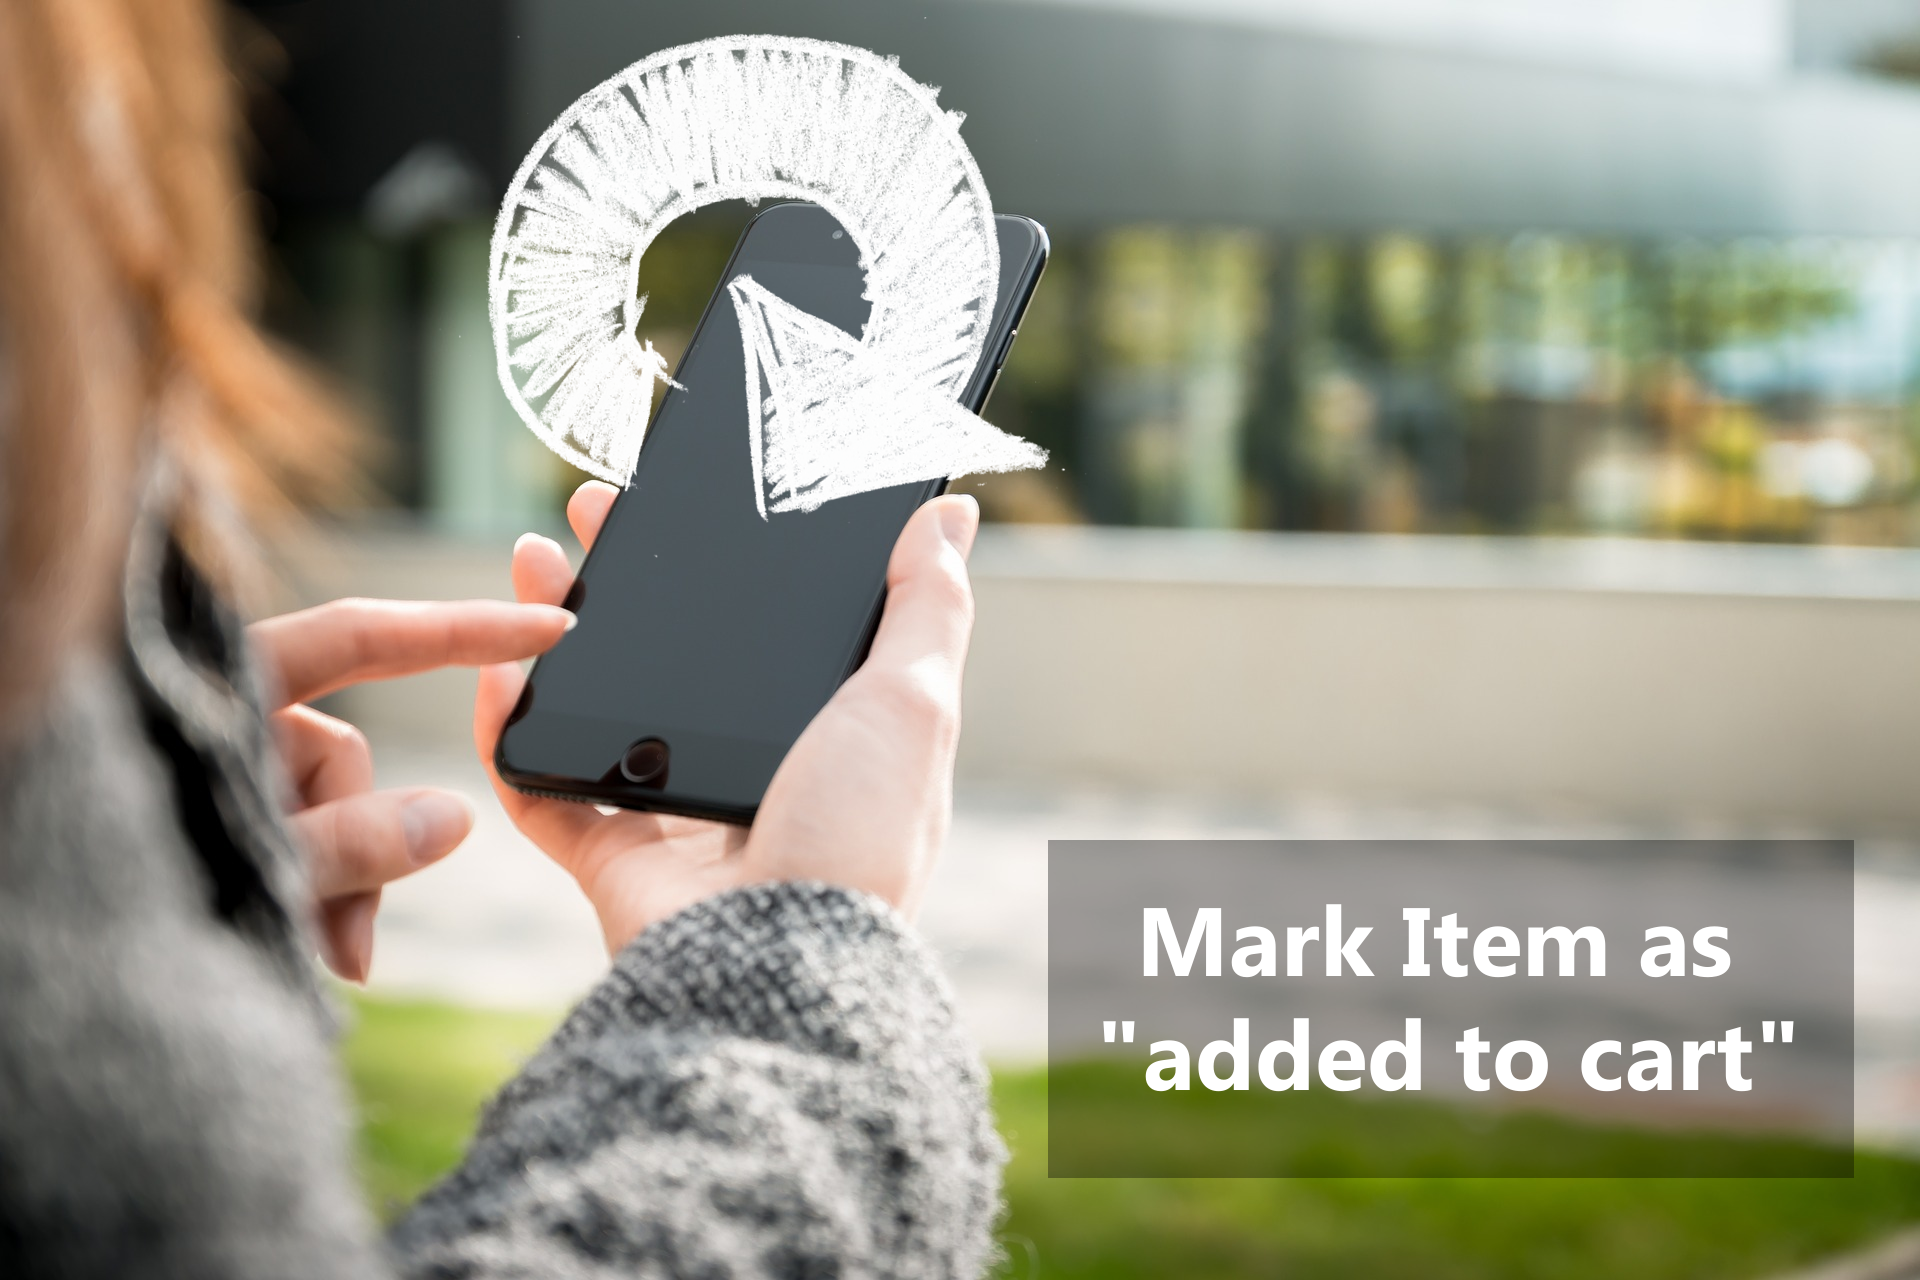
\includegraphics[width=\textwidth]{res/gestures/addToCart.png}
\caption{Add Item to Cart}
\label{fig:gestureAdd}
\end{subfigure} \hspace{0.05\textwidth}
\begin{subfigure}{0.475\textwidth}
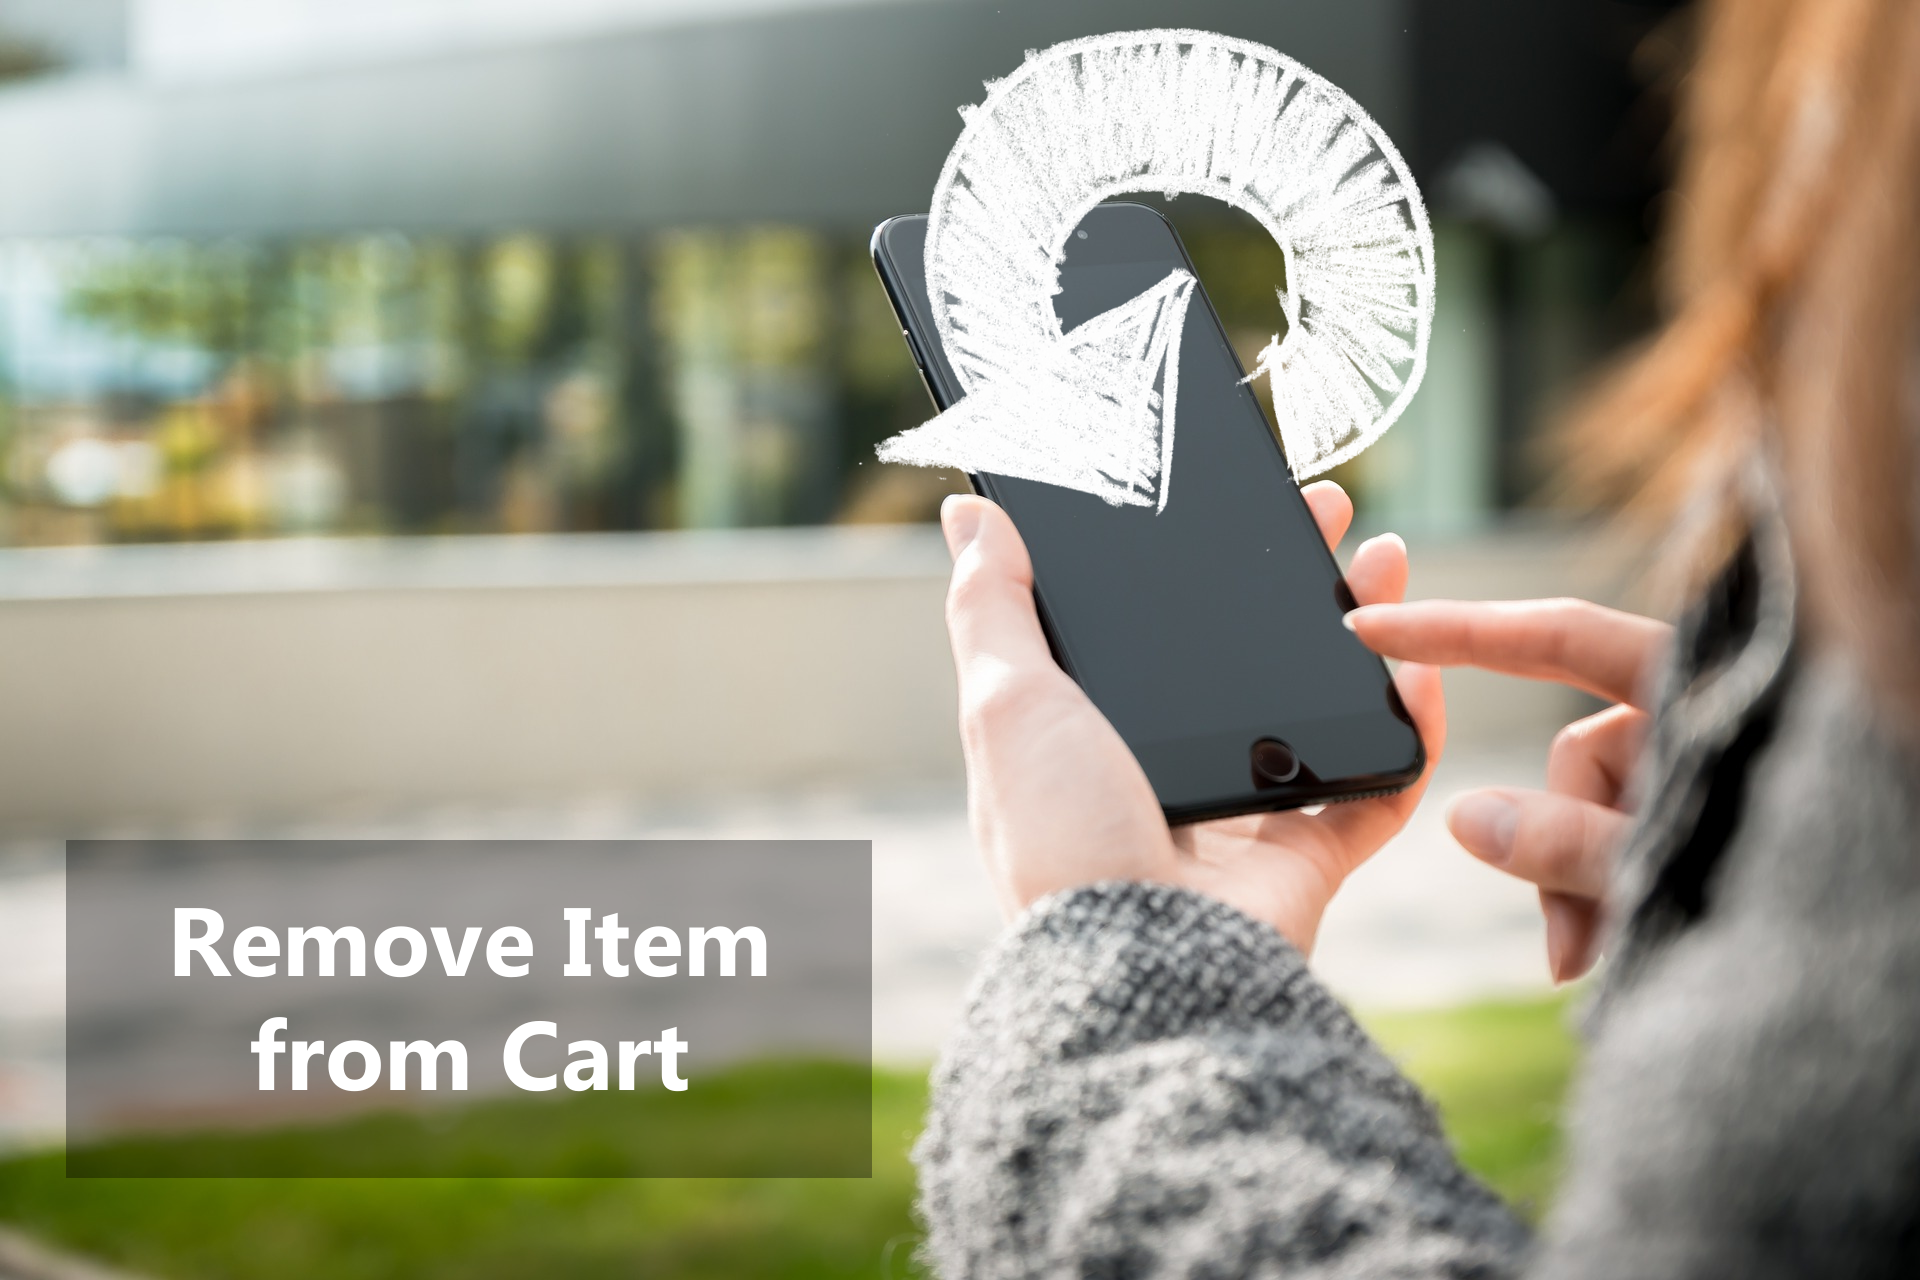
\includegraphics[width=\textwidth]{res/gestures/removeFromCart.png}
\caption{Switch Item}
\label{fig:gestureRemove}
\end{subfigure}
\caption{Gestures to Recognize}
\label{fig:gesturesToRecognize}
\end{figure}